\section{Datos disponibles}

Esta sección describe las distintas fuentes de datos consideradas en el estudio. Los datos de interés pueden ser clasificados en tres categorías. En primer lugar, se busca caracterizar a la población de la Región Metropolitana, en términos etarios y socioeconómicos. Esto se logra mediante el Censo 2017 y el Índice de Prioridad Social 2019.

En segundo lugar, se quiere conocer el comportamiento de la población, específicamente su uso del tiempo. Se ha relacionado previamente \cite{Munizaga2011}\cite{Kitamura1988}\cite{Axhausen1992} el uso del tiempo y los viajes, lo que lleva considerar datos de movilidad. La Encuesta Origen Destino Santiago 2012 es una fuente bastante rica en ese sentido; provee información desagregada de viajes y sus propósitos. Datos más actualizados que capturan las variaciones debido a la pandemia son el Uso de infraestructura de telecomunicaciones y los Informes de Movilidad Local sobre Covid-19.

Finalmente, se requieren datos para entender el avance de la pandemia. Datos-COVID19, un repositorio mantenido por la Mesa de Datos del Ministerio de Ciencia, Tecnología, Conocimiento e Innovación, contiene distintas series de tiempo de casos confirmados, hospitalizados, fallecidos, vacunados en el país, con distintos niveles de agregación.

% Para cada base de datos: 
% - Institución que la recopila 
% - Resumen de la metodología 
% - Datos que contiene 
% - Algunos resultados que sean relevantes para el trabajo 
% - Datos que sean de particular interés

%\noindent \textbf{Censo 2017}
\subsection{Censo 2017}

El Censo de Población y Vivienda 2017 fue un proceso liderado por el Instituto Nacional de Estadística (INE), y permitió contar y caracterizar a 17.574.003 personas y 6.499.355 viviendas en todo el territorio nacional.
% Podría definir aquí zona censal, lo usan la EOD y los de movilidad del ISCI.
Para el levantamiento del Censo del año 2017 y la desagregación de los datos censales se utiliza  en primer lugar la División Política Administrativa del país; regiones y comunas. Luego, el territorio de cada comuna se divide en distritos censales, los que pueden ser urbanos, rurales o mixtos. A su vez, en el área urbana se reconocen zonas censales, las que están compuestas de manzanas, y en el área rural, localidades.

Del Censo es de interés la población de la Región Metropolitana, desagregada por zona censal o comuna, sexo y edad. \\


%\noindent \textbf{\'Indice de prioridad social (IPS) 2019}
\subsection{\'Indice de prioridad social (IPS) 2019}


La Secretaría Regional Ministerial de Desarrollo Social y Familia de la Región Metropolitana de Santiago propone en \cite{SEREMIRM2019} una metodología que permite comparar las comunas respecto de sus niveles de desarrollo socioeconómico. El Índice de Prioridad Social (IPS) es un indicador compuesto que contempla ingresos, educación y salud. Se trata de un índice sintético cuyo valor numérico permite dimensionar el nivel de vida alcanzado por la población de una comuna, relativo al de las demás. \\ 


%\noindent \textbf{Encuesta Origen-Destino Santiago 2012}
\subsection{Encuesta Origen-Destino Santiago 2012}

Las Encuestas de Movilidad constituyen la principal fuente de información utilizada en todo proceso de planificación de los sistemas de transporte. Éstas entregan antecedentes relevantes sobre los patrones de movilidad de una determinada ciudad y proporcionan los datos requeridos para la calibración de los modelos de análisis de transporte. [link] %http://www.sectra.gob.cl/encuestas_movilidad/encuestas_movilidad.htm 
Estas encuestas son realizadas por el Programa de Vialidad y Transporte Urbano SECTRA, de la Subsecretaría de Transportes del Ministerio de Transportes y Telecomunicaciones (MTT), un organismo técnico especializado en planificación de transporte [link]. Se realizan cada diez años en las ciudades más grandes del país [Fuente requerida].
%http://www.sectra.gob.cl/quienes_somos/que_es_sectra.htm]

En la Encuesta Origen-Destino 2012 se recopiló información de los residentes de 18.000 hogares de Santiago, seleccionados aleatoriamente, durante el periodo comprendido entre julio de 2012 y noviembre de 2013. Su objetivo fue conocer las características de los viajes que se realizan en la ciudad y de quienes los efectúan. La encuesta se realizó mediante entrevista personal y los datos fueron recolectados en días hábiles y fines de semana, tanto en temporada normal como estival. En total se encuestaron alrededor de 60.000 personas (\cite{SECTRA2014})

% Qué información contiene la encuesta 

Como resultado, se cuenta con una base de datos con información de cada hogar, de las personas encuestadas y de los viajes realizados. Para cada hogar se cuenta con la fecha y temporada en que se realizó la encuesta, la ubicación geográfica, numero de personas que lo habitan e ingresos. De cada persona se conoce el hogar al que pertenece y la relación que tiene con el resto de moradores, sexo, edad, ocupación y tramo de ingresos. De cada viaje se conoce la persona que lo realizó, la zona censal de origen y destino, la hora de inicio y fin del viaje, los medios de transporte usados y el propósito del viaje. Se conocen todos los viajes realizados por cada persona.\\

% Aquí podría agregar imágenes de algunos análisis hechos a la encuesta 



%\noindent \textbf{Uso de infraestructura de telecomunicaciones}
\subsection{Uso de infraestructura de telecomunicaciones}\label{data:isci}

% Acerca de los proveedores
El Instituto Sistemas Complejos de Ingeniería (ISCI), que agrupa a un conjunto de investigadores de varias universidades de Chile con el objeto de generar trabajo científico y desarrollar soluciones para problemas complejos de ingeniería [link]
% Sus investigadores desarrollan proyectos en las áreas de la Gestión de Operaciones, Ingeniería de Transporte, Optimización y Energía, y otras como Organización Industrial y Medioambiente. Estas áreas comparten herramientas analíticas básicas y se complementan disciplinariamente. 
%[Link ing ISCI, http://ingenieria.uchile.cl/investigacion/centros-y-programas/88242/instituto-sistemas-complejos-de-ingenieria]
, en conjunto con Entel Ocean, la Unidad Digital de Entel, 
compañía de tecnología y telecomunicaciones, recopilaron información acerca del uso de infraestructura de telecomunicaciones, con datos agrupados a nivel de zona censal [link].
%Entel:  https://informacioncorporativa.entel.cl/nuestra-compania

% Acerca de la metodologia 
La información disponible les permitió deducir la zona hogar, en donde las personas se encuentran frecuentemente en horarios no laborales. Para cada día laboral (lunes a viernes), determinaron el flujo desde cada zona hogar a otras zonas, durante horarios de trabajo. Estos flujos pueden ser dentro de la misma comuna o a otras comunas, y fueron considerados un proxy de la movilidad en Santiago. % Luego, tomaron promedios semanales a nivel de comuna (excluyendo fines de semana) de esos flujos 
Las dos primeras semanas de marzo del 2020, antes de la declaración de la fase 2 de pandemia por COVID-19 en Chile, fueron consideradas como semanas "base”, siendo una aproximación para la movilidad usual de cada zona \cite{Olivares2020}. Los cambios en movilidad por zona con respecto a esa movilidad base fueron reportados para cada semana, y se encuentran disponibles en el repositorio de la Mesa de Datos del Ministerio de Ciencia, Tecnología, Conocimiento e Innovación [link github]. 
%Datos en https://github.com/MinCiencia/Datos-COVID19/tree/master/output/producto51 
La versión completa de estos datos, que contiene información tanto del origen como del destino de los transeúntes, fue analizada en \cite{Carranza2020}. La versión pública de estos datos, sin embargo, solo contiene la movilidad de entrada y salida de cada zona censal/comuna (es posible saber cuánta gente sale y entra a una zona censal o comuna pero no hacia dónde va). 


\begin{figure}[h]
\centering
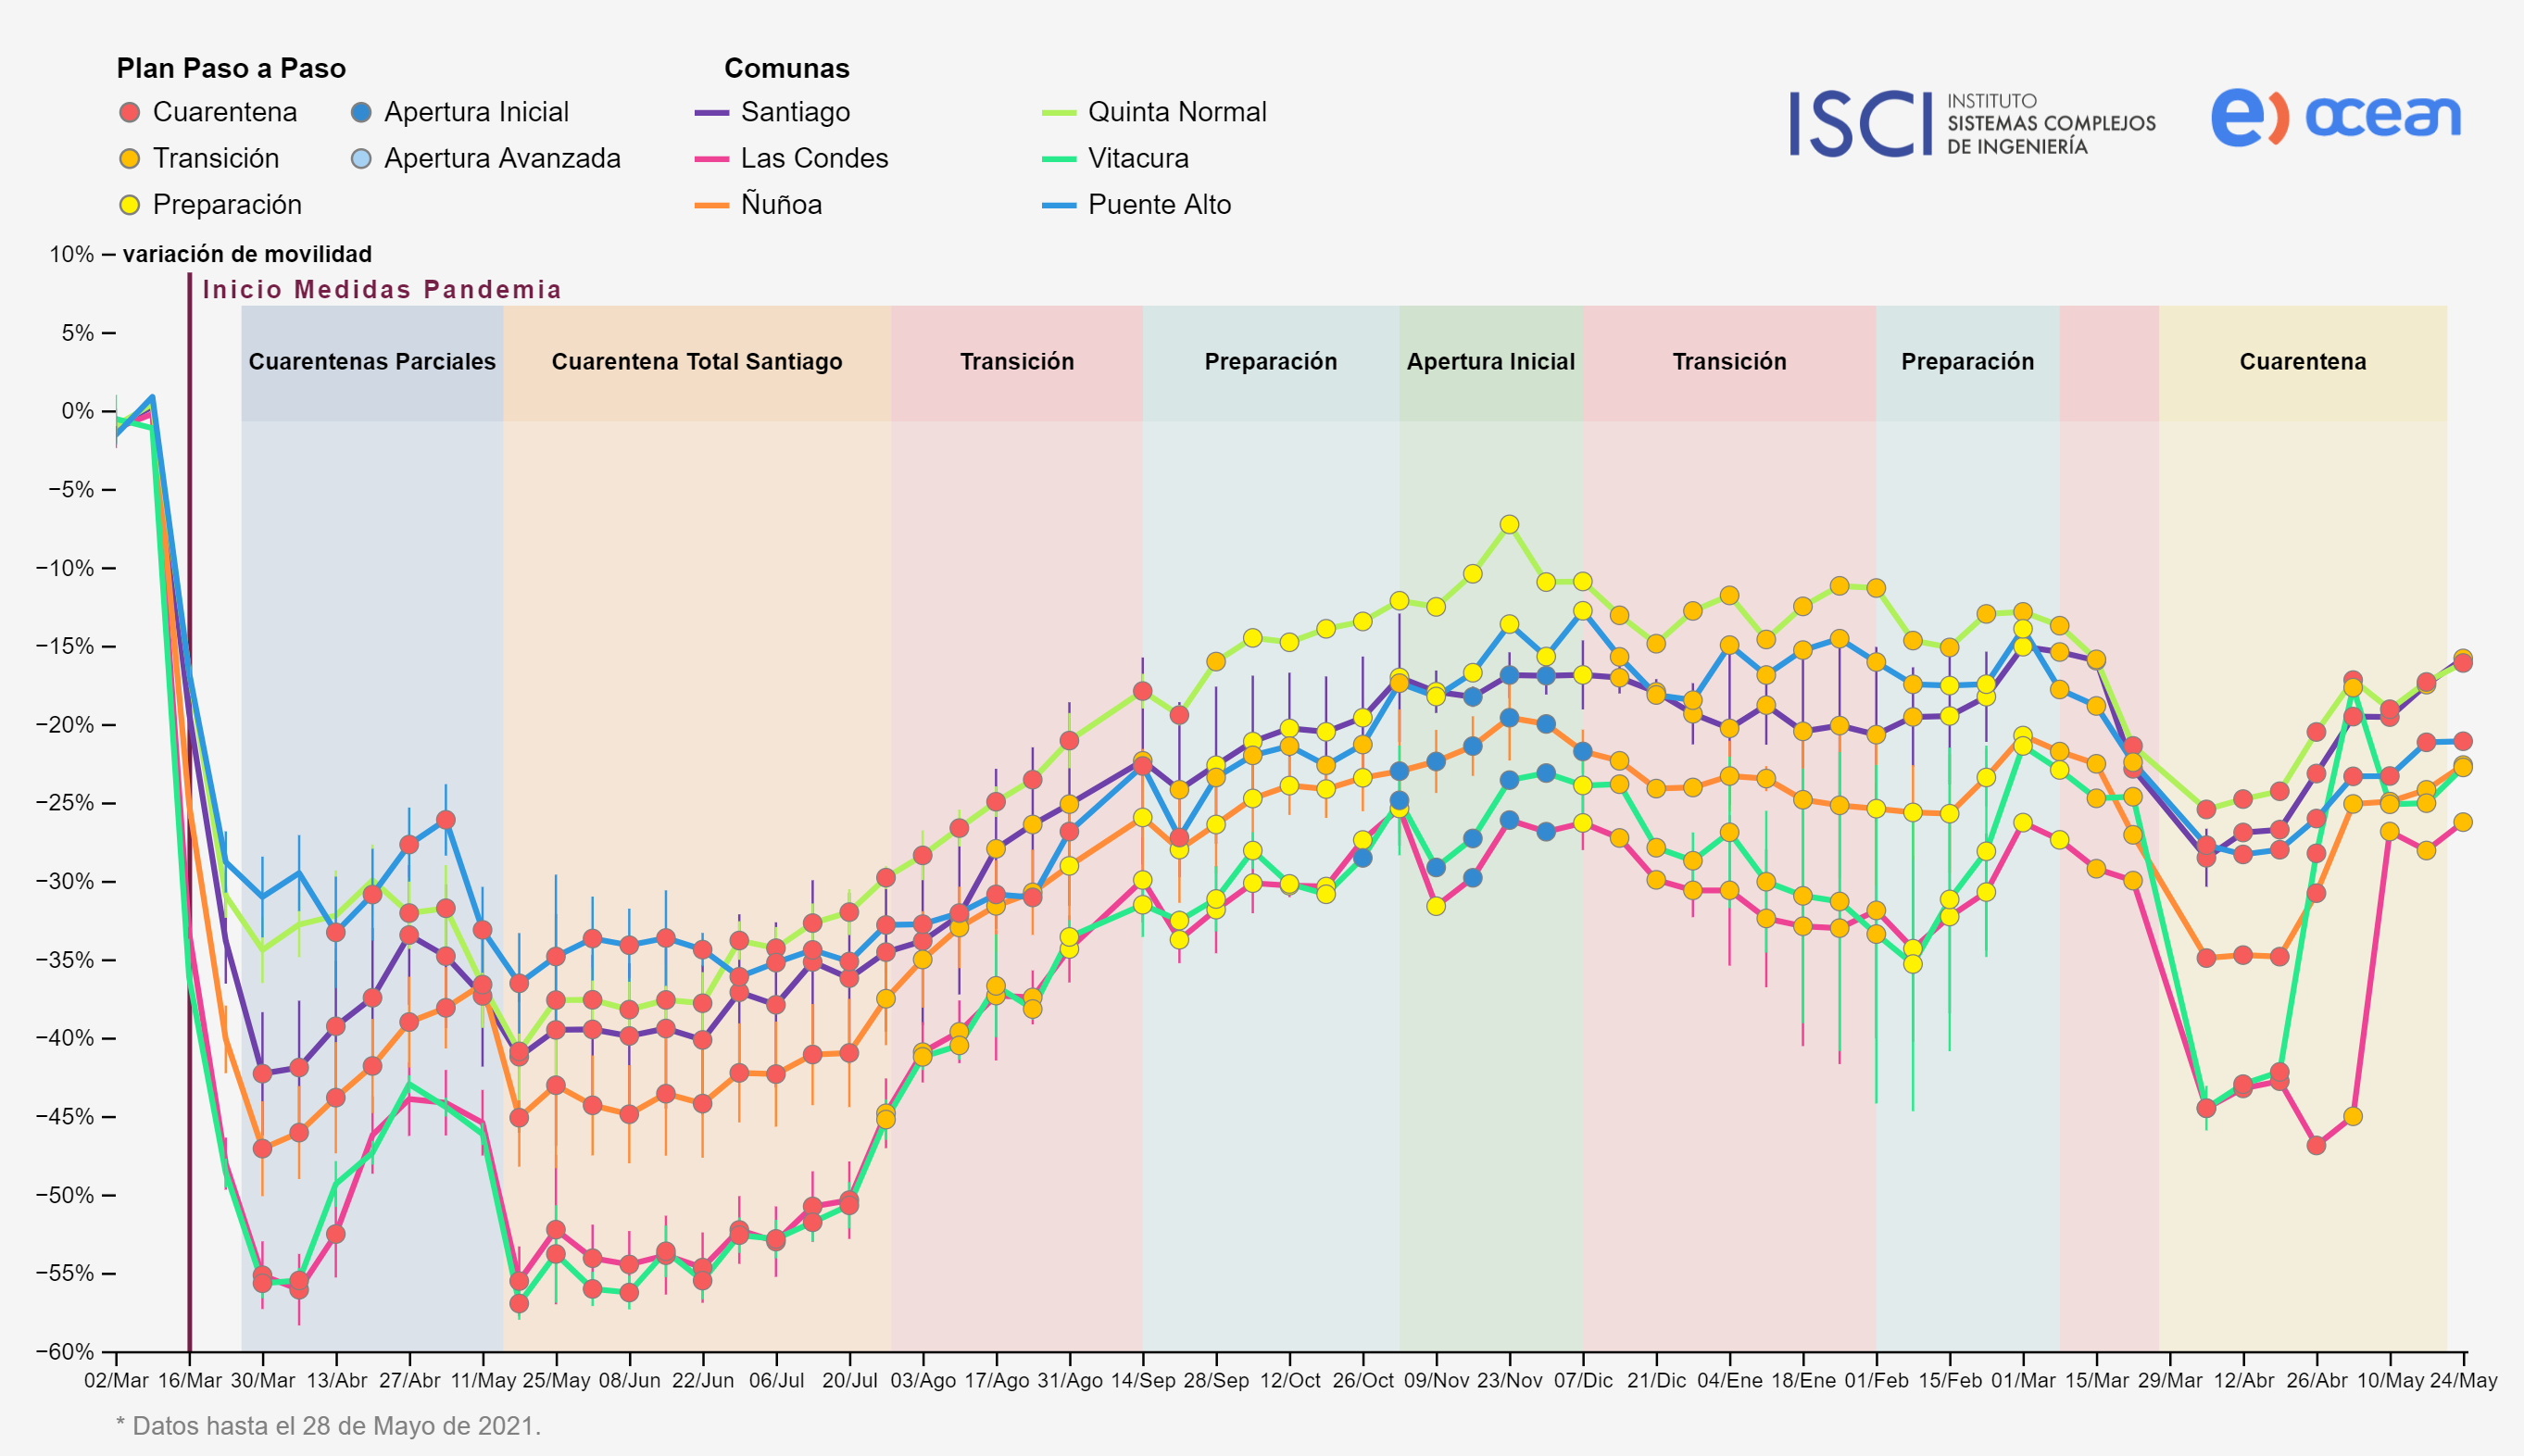
\includegraphics[width=\textwidth]{img/metodologia/datos/ISCI-movilidad-RM.png}
\caption{Variación en la movilidad de cinco comunas de la Región Metropolitana. Fuente: ISCI Covid Analytics.}
\label{img:ISCI-movilidad-RM}
\end{figure}


%\noindent \textbf{Informes de Movilidad Local sobre Covid-19}
\subsection{Informes de Movilidad Local sobre Covid19}

Reportados por Google a partir de datos anonimizados que usan en servicios como Google Maps. Pretenden proporcionar información a las autoridades sanitarias de los cambios en la movilidad como consecuencia de las distintas políticas de contención del Covid19. Las series de tiempo se encuentran clasificadas en varias categorías: tiendas y ocio, supermercados y farmacias, parques, estaciones de transporte, lugares de trabajo y zonas residenciales.

\begin{figure}[h]
\centering
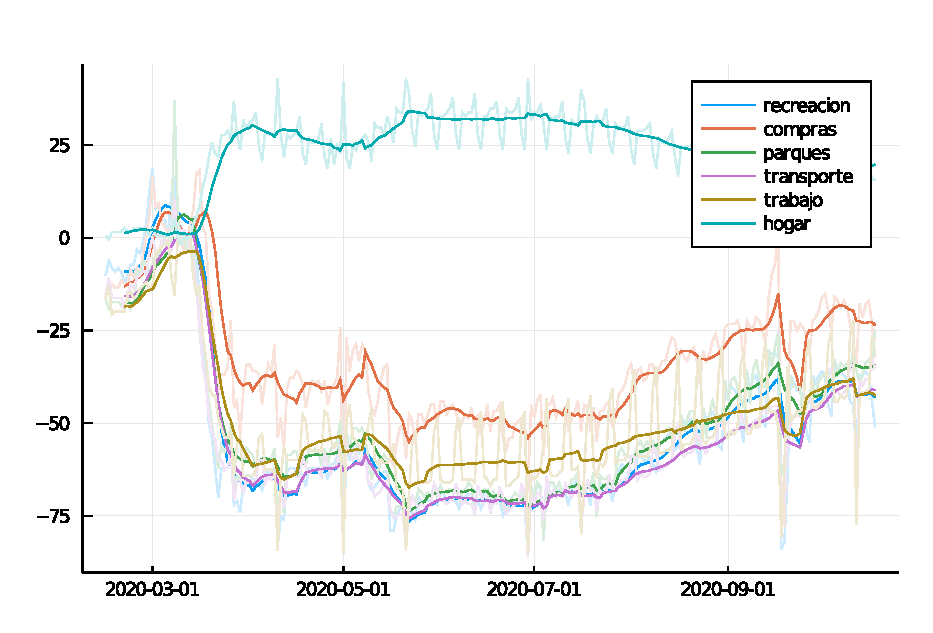
\includegraphics[width=\textwidth]{img/metodologia/datos/explorar_movilidad_google_6_1.eps}
\caption{Variación en la movilidad agregada por actividad en la Región Metropolitana y media móvil de 7 días. Fuente: Elaboración propia con datos de Google.}
\label{img:google-movilidad-RM}
\end{figure}

\subsection{Datos-COVID19}

La Mesa de Datos COVID-19 liderada por el Ministerio de Ciencia, Tecnología, Conocimiento e Innovación busca proveer de información del país durante la pandemia, con el fin de promover el uso de datos para investigación científica, clínica y para soluciones innovadoras. Dispone de datos documentados del Ministerio de Salud (MINSAL) y de otras fuentes.

% datos disponibles
La información está organizada en distintos \textit{Data Products}. Existen series de tiempo de casos confirmados, hospitalizados, UCI, conectados a ventilación mecánica, fallecidos, cantidad de exámenes PCR realizados, nacimientos y fallecimientos, cuarentenas, etc. 

\begin{figure}[h]
\centering
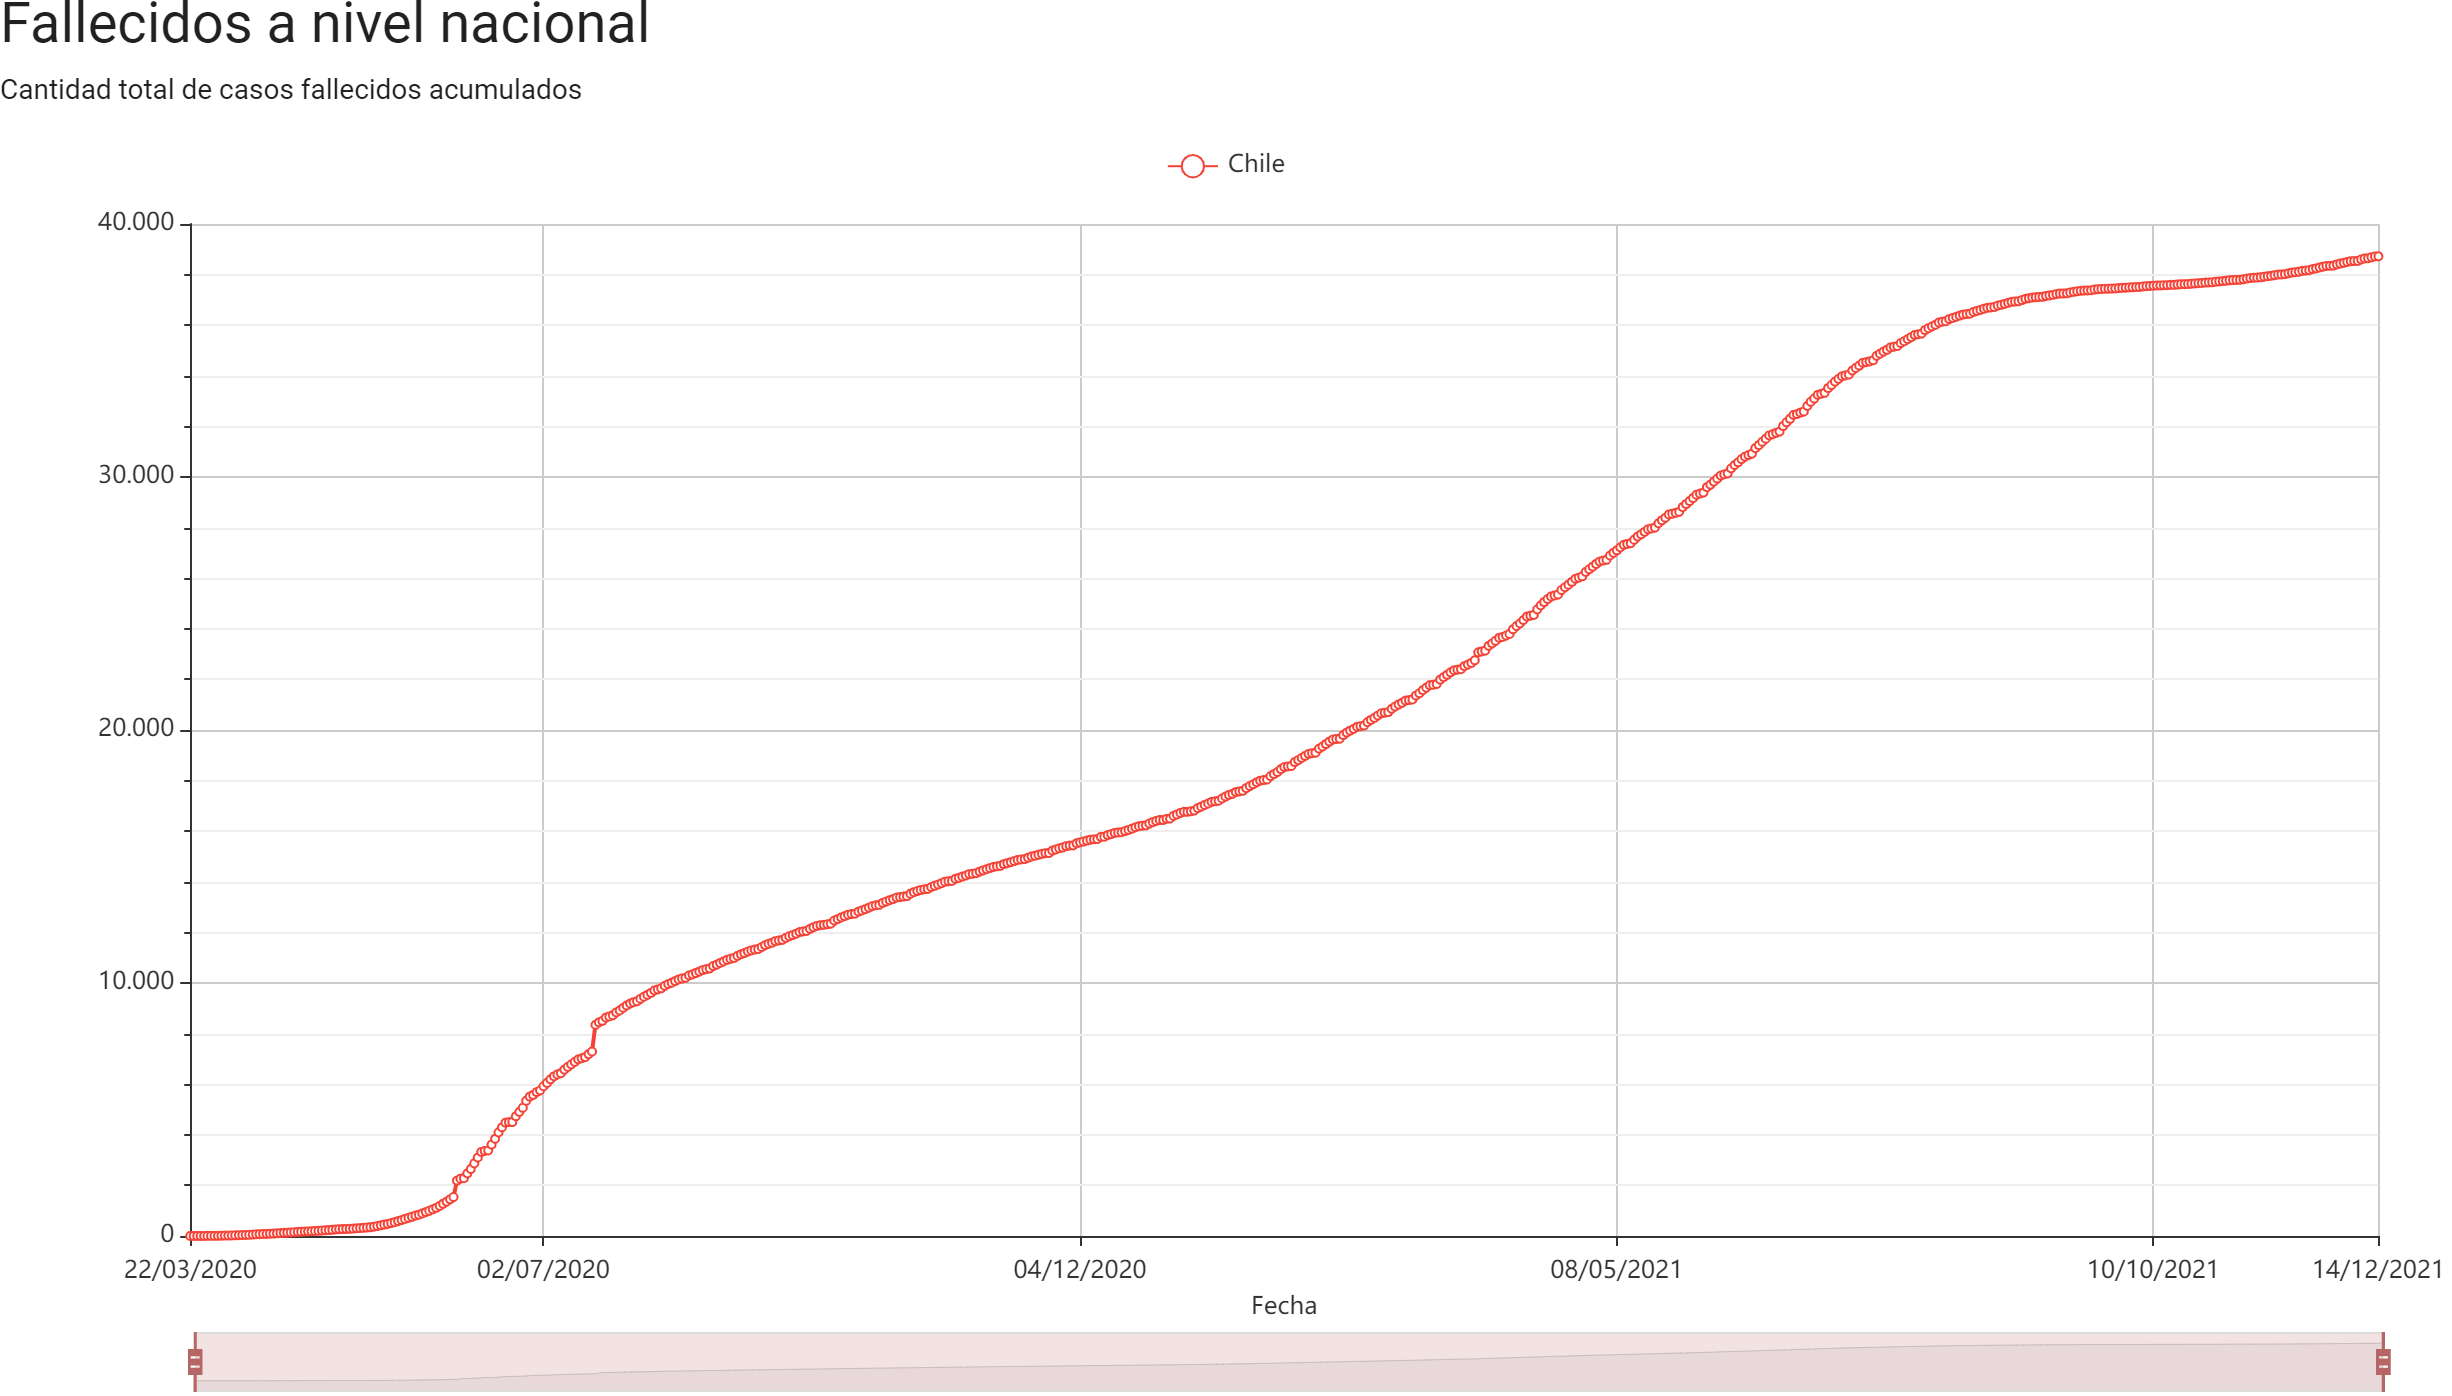
\includegraphics[width=\textwidth]{img/metodologia/datos/fallecidos_nacional.png}
\caption{Total de casos fallecidos por Covid19 acumulados a nivel nacional. Fuente: Centro de Modelamiento Matemático  con Datos-COVID19.}
\label{img:cmm-fallecidos}
\end{figure}

